Seja $S_i$ a área de intersecção do triângulo com a região de pontuação da
$i$-ésima semicircunferência (de forma que a resposta é $\displaystyle \sum_{i=1}^{N} v_i \times S_i$).

Primeiramente, note que $S_i$ é igual à área de intersecção do triângulo com o
$i-$ésimo semicírculo, subtraído da área de intersecção do triângulo com o
$(i-1)-$ésimo semicírculo:

\begin{center}
    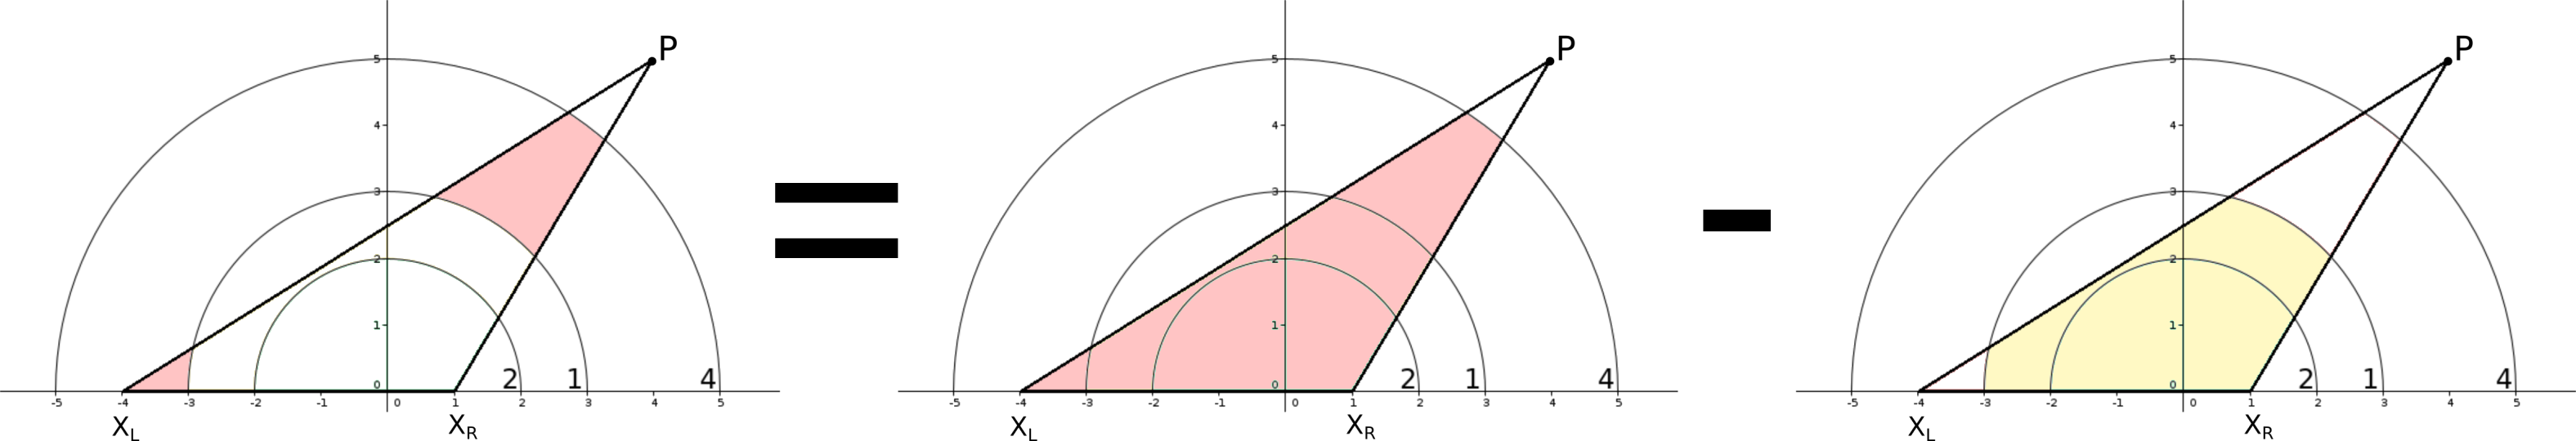
\includegraphics[scale=0.2]{arremesso/editorial-imgs/sub.png}
\end{center}

Desta forma, o problema é reduzido a determinar a área $A$ de intersecção de um
triângulo com um semicírculo.

Tal área pode ser dada pelas áreas de alguns triângulos e de
alguns setores circulares, de acordo com os seguintes casos (sejam $L=(X_L,0)$,
        $R=(X_R,0)$ e $O=(0,0)$):

\begin{center}
    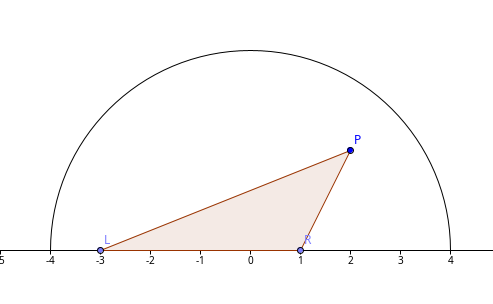
\includegraphics[scale=1.7]{arremesso/editorial-imgs/caso1.png}\\
    Caso 1: $P$, $L$ e $R$ dentro do semicírculo.\\$A = \Delta LRP$
\end{center}

\begin{center}
    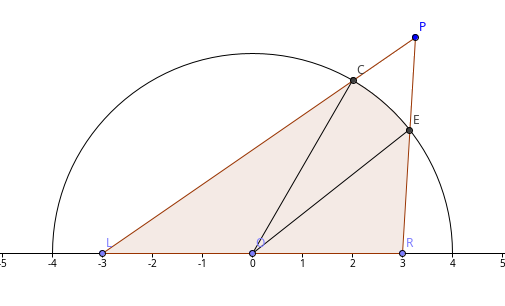
\includegraphics[scale=1.7]{arremesso/editorial-imgs/caso2.png}\\
    Caso 2: $P$ fora; $L$ e $R$ dentro do semicírculo.\\$A = \Delta LCO + \measuredangle OCE + \Delta ERO$
\end{center}

\begin{center}
    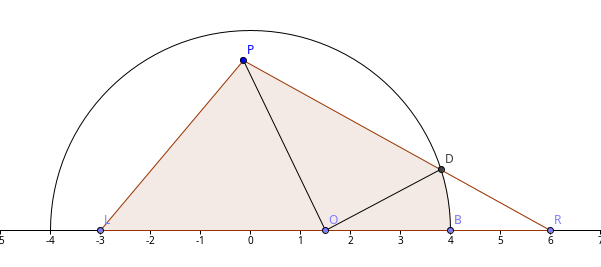
\includegraphics[scale=1.7]{arremesso/editorial-imgs/caso3.png}\\
    Caso 3: $R$ fora; $L$ e $P$ dentro do semicírculo.\\$A = \Delta LPO + \Delta PDO + \measuredangle ODB$
\end{center}

\begin{center}
    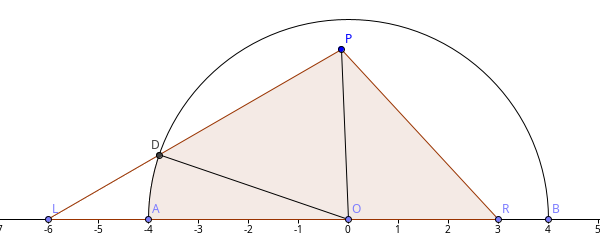
\includegraphics[scale=1.7]{arremesso/editorial-imgs/caso4.png}\\
    Caso 4: $L$ fora; $R$ e $P$ dentro do semicírculo.\\$A = \measuredangle OAD + \Delta PDO + \Delta PRO$
\end{center}

\begin{center}
    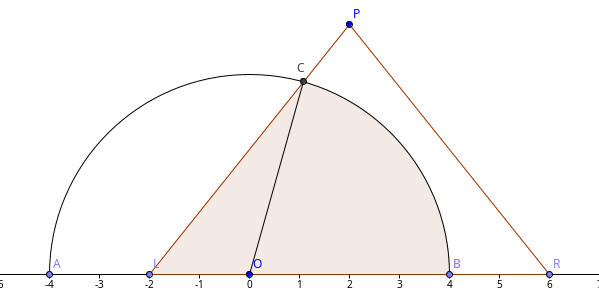
\includegraphics[scale=1.7]{arremesso/editorial-imgs/caso51.png}\\
    Caso 5.1: $R$ e $P$ fora; $L$ dentro do semicírculo; $\overline{PR}$ não
    intersecta a semicircunferência.\\$A = \Delta CLO + \measuredangle OCB$
\end{center}

\begin{center}
    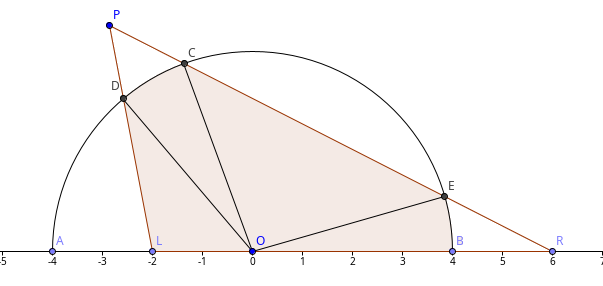
\includegraphics[scale=1.7]{arremesso/editorial-imgs/caso52.png}\\
    Caso 5.2: $R$ e $P$ fora; $L$ dentro do semicírculo; $\overline{PR}$ intersecta a semicircunferência.\\
    $A = \Delta DLO + \measuredangle ODC + \Delta CEO + \measuredangle OEB$
\end{center}

\begin{center}
    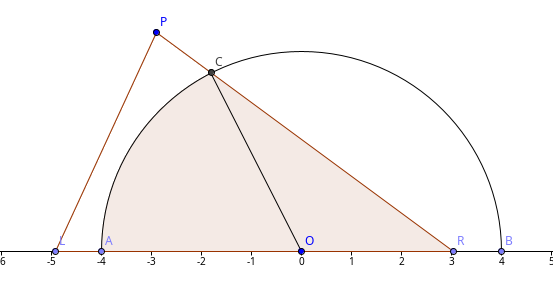
\includegraphics[scale=1.7]{arremesso/editorial-imgs/caso61.png}\\
    Caso 6.1: $L$ e $P$ fora; $R$ dentro do semicírculo; $\overline{PL}$ não intersecta a semicircunferência.\\
    $A = \measuredangle OAC + \Delta CRO$
\end{center}

\begin{center}
    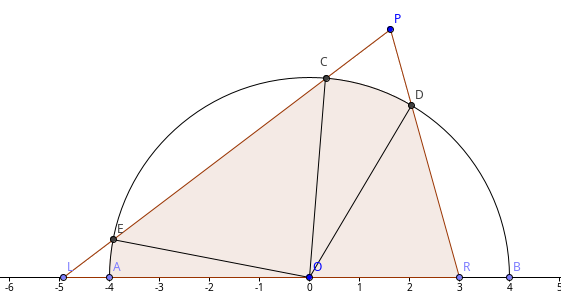
\includegraphics[scale=1.7]{arremesso/editorial-imgs/caso62.png}\\
    Caso 6.2: $L$ e $P$ fora; $R$ dentro do semicírculo; $\overline{PL}$ intersecta a semicircunferência.\\
    $A = \measuredangle OEA + \Delta ECO + \measuredangle OCD + \Delta ODR$
\end{center}

\begin{center}
    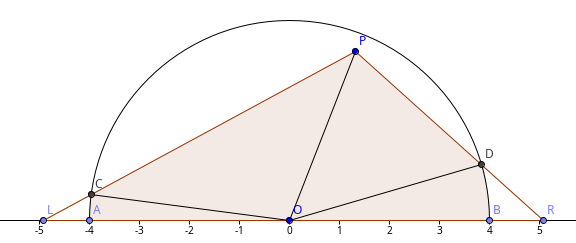
\includegraphics[scale=1.7]{arremesso/editorial-imgs/caso7.png}\\
    Caso 7: $L$ e $R$ fora; $P$ dentro do semicírculo.\\
    $A = \measuredangle OAC + \Delta PCO + \Delta PDO + \measuredangle ODB$
\end{center}

\begin{center}
    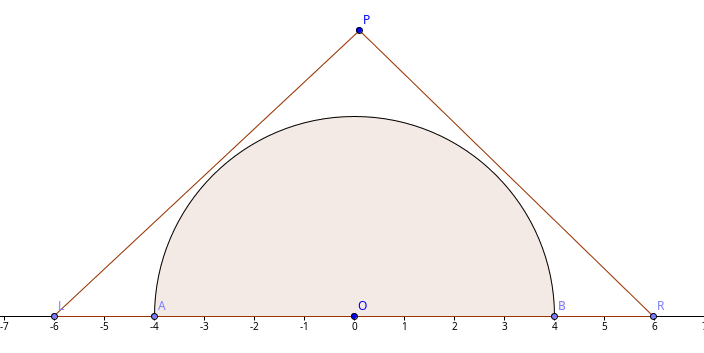
\includegraphics[scale=1.7]{arremesso/editorial-imgs/caso81.png}\\
    Caso 8.1: $P$, $L$ e $R$ fora do semicírculo; $\overline{PL}$ e $\overline{PR}$ não intersectam a semicircunferência.\\
    $A = \measuredangle OAB = \displaystyle\frac{\pi r^2}{2}$
\end{center}

\begin{center}
    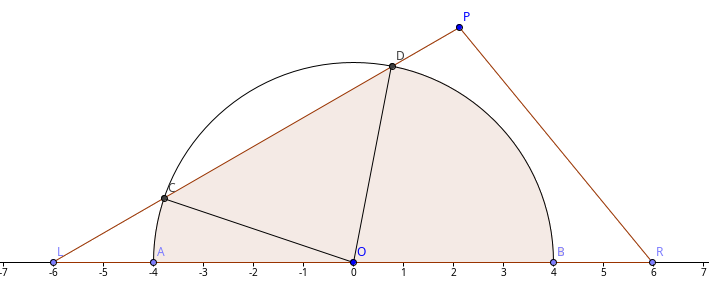
\includegraphics[scale=1.7]{arremesso/editorial-imgs/caso82.png}\\
    Caso 8.2: $P$, $L$ e $R$ fora do semicírculo; $\overline{PL}$ intersecta; $\overline{PR}$ não intersecta a semicircunferência.\\
    $A = \measuredangle OAC + \Delta CDO + \measuredangle ODB$
\end{center}

\begin{center}
    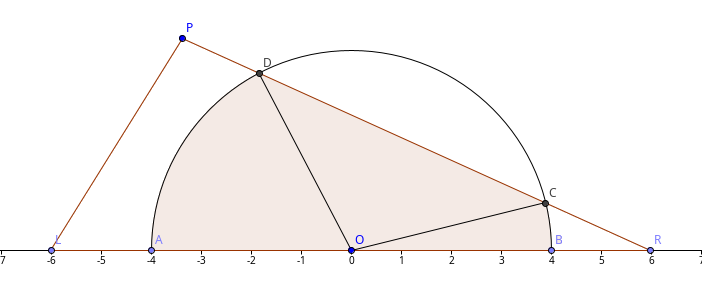
\includegraphics[scale=1.7]{arremesso/editorial-imgs/caso83.png}\\
    Caso 8.3: $P$, $L$ e $R$ fora do semicírculo; $\overline{PR}$ intersecta; $\overline{PL}$ não intersecta a semicircunferência.\\
    $A = \measuredangle OAD + \Delta CDO + \measuredangle OCB$
\end{center}

\begin{center}
    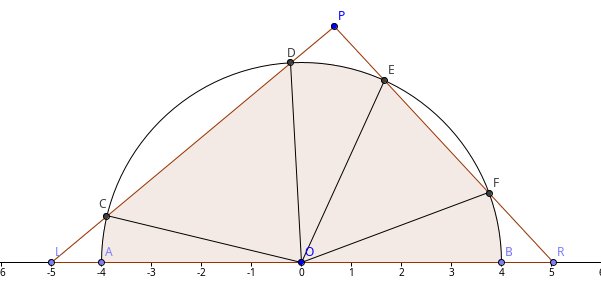
\includegraphics[scale=1.7]{arremesso/editorial-imgs/caso84.png}\\
    Caso 8.4: $P$, $L$ e $R$ fora do semicírculo; $\overline{PL}$ e $\overline{PR}$ intersectam a semicircunferência.\\
    $A = \measuredangle OAC + \Delta CDO + \measuredangle ODE + \Delta EFO + \measuredangle OFB$
\end{center}

Note que, para determinar os triângulos e setores circulares, se faz necessário
conhecer diversas operações de geometria, como:
intersecção de reta com círculo;
área de triângulo dados três vértices;
ângulo entre dois segmentos de reta;
área de setor circular;
etc.

Recomenda-se fortemente ter uma biblioteca de Geometria 2D em suas anotações
contendo uma grande coleção de operações. Suas implementações ficam como exercício para o
leitor.

Complexidade total: $O(N)$.
